%%%%%%%%%%%%%%%%%%%%%%%%%%%%%%%%%%%%%%%%%
% Sullivan Business Report
% LaTeX Template
% Version 1.0 (May 5, 2022)
%
% This template originates from:
% https://www.LaTeXTemplates.com
%
% Author:
% Vel (vel@latextemplates.com)
%
% License:
% CC BY-NC-SA 4.0 (https://creativecommons.org/licenses/by-nc-sa/4.0/)
%
%%%%%%%%%%%%%%%%%%%%%%%%%%%%%%%%%%%%%%%%%

%----------------------------------------------------------------------------------------
%	CLASS, PACKAGES AND OTHER DOCUMENT CONFIGURATIONS
%----------------------------------------------------------------------------------------

\documentclass[
	a4paper, % Paper size, use either a4paper or letterpaper
	12pt, % Default font size, the template is designed to look good at 12pt so it's best not to change this
	%unnumberedsections, % Uncomment for no section numbering
]{CSSullivanBusinessReport}

%\addbibresource{sample.bib} % BibLaTeX bibliography file

%----------------------------------------------------------------------------------------
%	REPORT INFORMATION
%----------------------------------------------------------------------------------------

\reporttitle{SafeSign} % The report title to appear on the title page and page headers, do not create manual new lines here as this will carry over to page headers

\reportsubtitle{Sistema empotrado de establecimiento de \\ velocidad máxima 
con respecto a las condiciones meteorológicas} % Report subtitle, include new lines if needed

\reportauthors{José Alfredo Lopez José, \\ Jesús Carrascosa Carro, \\ José Pablo Ruiz Pérez, \\ Yeray Rincón Cardoso } % Report authors/group/department, include new lines if needed
%TODO: cambiar si fuera nencesario
\reportdate{2024-03-04} % Report date, include new lines for additional information if needed

\rightheadercontent{
\includegraphics[width=3cm]{creodocs_logo.pdf}} % The content in the right header, you may want to add your own company logo or use your company/department name or leave this command empty for no right header content
\renewcommand{\contentsname}{Índice}

%----------------------------------------------------------------------------------------

\begin{document}

%----------------------------------------------------------------------------------------
%	TITLE PAGE
%----------------------------------------------------------------------------------------

\thispagestyle{empty} % Suppress headers and footers on this page

\begin{fullwidth} % Use the whole page width
	\vspace*{-0.075\textheight} % Pull logo into the top margin
	
	\hfill
\includegraphics[width=5cm]{creodocs_logo.pdf} % Company logo

	\vspace{0.15\textheight} % Vertical whitespace

	\parbox{0.9\fulltextwidth}{\fontsize{50pt}{52pt}\selectfont\raggedright\textbf{\reporttitle}\par} % Report title, intentionally at less than full width for nice wrapping. Adjust the width of the \parbox and the font size as needed for your title to look good.
	
	\vspace{0.03\textheight} % Vertical whitespace
	
	{\LARGE\textit{\textbf{\reportsubtitle}}\par} % Subtitle
	
	\vfill % Vertical whitespace
	
	{\Large\reportauthors\par} % Report authors, group or department
	
	\vfill\vfill\vfill % Vertical whitespace
	
	{\large\reportdate\par} % Report date
\end{fullwidth}

\newpage

%----------------------------------------------------------------------------------------
%	DISCLAIMER/COPYRIGHT PAGE
%----------------------------------------------------------------------------------------

\thispagestyle{empty} % Suppress headers and footers on this page

\begin{twothirdswidth} % Content in this environment to be at two-thirds of the whole page width
	\footnotesize % Reduce font size
	
	
	\subsection*{Copyright}
	
	\textcopyright~[2024] [LinterniTek S.Coop.And] 
	
	%TODO el copy
	\subsection*{Información de Contacto}
	% TODO Poner info de contacto
	E.T.s. De Ing. Informática\\
	Av. Reina mercedes S/N\\
    Sevilla, España\\
	41005\\
	
	NIF: F-1234567-E
	
	Correo electrónico: \href{mailto:contacto@linternitek.com}{contacto@linternitek.com}.
	
	\vfill % Push the following down to the bottom of the page
	\subsection*{Acerca del documento}
	\subsubsection*{Registro de Cambios}
	
	\scriptsize % Reduce font size further
	
	\begin{tabular}{@{} L{0.05\linewidth} L{0.15\linewidth} L{0.6\linewidth} @{}} % Column widths specified here, change as needed for your content
		\toprule % Modificar
		v1.0 & 2024-02-05 & Creada la plantilla \\
		v1.1 & 2024-02-27 &  Pequeños cambios en el contexto\\ 
		v1.2 & 2024-03-01 & Modificada la información de contacto\\
		\bottomrule
	\end{tabular}
    \subsubsection*{Estado del documento}
    \scriptsize
      
        \begin{tabular}{cc}
        \toprule
            Código& PGPI-LTK-SFSNG-MANDATO \\
             Estado& APROBADO\\
             Fecha& 2024-03-04 \\
             Versíon& 1.2\\
             \bottomrule
        \end{tabular}
       
    \subsubsection*{Distribución del documento}
        \begin{tabular}{|c|c|c|c|}
        \toprule
         \textbf{Acción} & \textbf{Nombre} &\textbf{Firma} & \textbf{Fecha}\\
         \midrule
         ELABORACIÓN & Jesús Carrascosa Carro & \textit{yisus }& 2024-03-01\\
         \midrule
         REVISIÓN & Jesús Carrascosa Carro & \textit{yisus} & 2024-03-02\\
         REVISIÓN & José Alfredo Lopez José & \textit{JoseAl} & 2024-03-02\\
         \midrule
         APROBACIÓN & Jesús Carrascosa Carro & yisus & 2024-03-04\\
         APROBACIÓN & José Alfredo Lopez José & \textit{JoseAl} & 2024-03-04\\
         APROBACIÓN & José Pablo Ruiz Pérez & \textit{RuizPerez} & 2024-03-04\\
         APROBACIÓN & Yeray Rincón Cardoso & \textit{yeray} & 2024-03-04\\
         \bottomrule
         
        \end{tabular}
\end{twothirdswidth}

\newpage

%----------------------------------------------------------------------------------------
%	TABLE OF CONTENTS
%----------------------------------------------------------------------------------------

\begin{twothirdswidth} % Content in this environment to be at two-thirds of the whole page width
	\tableofcontents % Output the table of contents, automatically generated from the section commands used in the document
\end{twothirdswidth}

\newpage

%----------------------------------------------------------------------------------------
%	SECTIONS
%----------------------------------------------------------------------------------------
\begin{fullwidth}
    

\section{Contexto}
\subsection{Sobre Nosotros}
Nuestra empresa, LinterniTek, se dedica al desarrollo de Sistemas Empotrados aplicados al ámbito de la automoción y la seguridad vial, con la misión de optimizar y mejorar la seguridad vial y la gestión del tráfico en tiempo real utilizando sistemas autónomos y conectados.  
\par
Esta propuesta de proyecto forma parte de la visión de la empresa de crear soluciones innovadoras para gestionar y adaptar las condiciones de las carreteras a las necesidades de los usuarios, de manera que se reduzca el riesgo de accidentes de tráfico y se mejore la fluidez del tráfico
\subsection{Sobre el problema }
En los últimos años en España, debido a las fluctuaciones extremas y rápidas del clima (que en caso de precipitaciones y neblina se traduce en una reducción de la visibilidad) y sumadas a la deficiente señalización, el estado de deterioro de algunas carreteras y la influencia de accidentes cercanos recientes lo que dificulta que los conductores puedan evaluar su entorno de manera adecuada, lo que a su vez lleva a comportamientos impredecibles. Esto ha llevado a un aumento en los accidentes de tráfico. Esta problemática se agravará a medida que el creciente cambio climático provoque una mayor impredecibilidad en las condiciones temporales, requiriendo una mayor capacidad de adaptación con menores márgenes de reacción. 
\par 
Con el fin de ilustrar la problemática, a continuación, se detallan diversos accidentes cuya causa principalmente fue la baja visibilidad: 
\begin{itemize}
    \item El martes 20 de marzo de 2024, sobre las 4 de la madrugada, ocurrió un fatal accidente en la autopista AP-4 que conecta Cádiz con Sevilla. Debido a la baja visibilidad y a una mala señalización, un camión (que además iba por encima del límite de velocidad permitido por el camión y por la autopista) embistió un control de la Guardia Civil situado en la salida a Utrera en sentido Sevilla matando a seis personas en el suceso.

    \item Unos días después, a la altura de la salida hacia el aeropuerto de Jerez y en sentido Sevilla, ocurrió otro accidente en el cual, debido a la lluvia intensa y a la velocidad que dicho conductor llevaba en el momento (más de 120 kilómetros por hora), acabó atravesando la mediana y casi llegando al carril contrario de la circulación.
\end{itemize}
\end{fullwidth}
\newpage
\begin{fullwidth}
    

\section{Alcance del proyecto}
\subsection{Objetivos}
El objetivo principal de este proyecto es llevar a cabo un sistema de señalización automático de la velocidad (denominado SafeSign) que tenga en cuenta diversos factores como pueden ser ambientales, lumínicos, tráfico, accidentales e incluso estadísticos para poder determinar una nueva velocidad máxima permitida y así avise a los conductores de los posibles peligros y de la nueva velocidad permitida mediante señales electrónicas dispuestas en puntos estratégicos de la carretera. Pretendiendo así lo siguiente:  
\begin{itemize}
    \item Poder asegurar que los usuarios puedan conducir de manera segura por una carretera independientemente de las condiciones en la que se encuentre la misma. 

    \item Proporcionar información a los usuarios que usen dicha carretera del estado en el que se encuentra.

    \item Realizar un control automático sobre la velocidad de las carreteras teniendo en cuenta los factores meteorológicos que haya. 

    \item  Reducir el número de accidentes de tráfico y victimas que puedan ocasionarse debido a las condiciones meteorológicas. 

    \item  Generar y proporcionar un corpus de datos que permitan llevar a cabo evaluaciones estadísticas y análisis a gran escala con Big Data e Inteligencia Artificial. 

    \item  Comercializar este sistema de forma internacional para así poder reducir a nivel mundial el número de accidentes de tráfico. 
\end{itemize}



\subsection{Alcance}
\subsubsection{Organizativo}

\subsubsection{Funcional}
\subsubsection{Temporal}

\subsection{Restricciones}
\subsection{Dependencias}
Este proyecto no depende de ningún proyecto previo

\end{fullwidth}
\section{Section Title} % Top level section

Lorem ipsum dolor sit amet, consectetur adipiscing elit. Aliquam auctor mi risus, quis tempor libero hendrerit at. Duis hendrerit placerat quam et semper. Nam ultricies metus vehicula arcu viverra, vel ullamcorper justo elementum. Pellentesque vel mi ac lectus cursus posuere et nec ex. Fusce quis mauris egestas lacus commodo venenatis. Ut at arcu lectus. Donec et urna nunc. Morbi eu nisl cursus sapien eleifend tincidunt quis quis est. Donec ut orci ex. Praesent ligula enim, ullamcorper non lorem a, ultrices volutpat dolor. Nullam at imperdiet urna. Pellentesque nec velit eget est pretium.\sidenote{This is a sidenote. This template features a large margin specifically so you can put notes, figures, tables and other things into it as additional material to the main content in the text block.}

Donec in elit ac ante vestibulum rhoncus. Pellentesque ligula tortor, aliquet malesuada nulla tristique vitae. Aliquam mi sem, varius eu pellentesque et, tristique nec quam. Vestibulum pellentesque in dui et venenatis. Sed malesuada elit pellentesque sapien aliquet porta. In at facilisis diam. Duis id ante tellus.\sidenote[][2cm]{This sidenote has been pushed down the page manually with an optional parameter, otherwise it would be right under the one above.} % This first optional argument to a sidenote is the symbol to use (leave this empty for automatic numbering) and the second is the vertical offset (positive is down, negative is up)

\subsection{Subsection Title} % Second level section

In diam libero, vulputate quis accumsan non, auctor in ipsum. Praesent cursus velit eget lacus sodales porta. Proin quis risus ut velit euismod scelerisque ut sed neque. Cras sagittis, dolor ac ullamcorper auctor, tortor dui facilisis diam, at sagittis nisi ipsum a neque. Nullam vel mattis nisi. Ut interdum ut diam at ornare. Nulla ultrices elit justo, vitae tristique massa vulputate sit amet.

\nonumsidenote{This sidenote isn't numbered in the text or margin. This is useful for notes that apply anywhere on the page instead of one particular place.}Vestibulum erat felis, cursus vitae convallis ac, commodo eu nisi. Nulla facilisi. Mauris dignissim nisi felis, a mollis ex accumsan vel. Suspendisse bibendum vitae nibh in suscipit. Vestibulum et finibus eros. Nulla facilisi. Cras luctus aliquam finibus. In nec justo nec orci malesuada faucibus.

\subsubsection{Subsubsection Title} % Third level section

\begin{fullwidth} % Use the whole page width
	\textit{This is an example of a full width paragraph\ldots} Curabitur id placerat orci. Vivamus pulvinar augue ac feugiat blandit. Donec in ultricies mi. Nam eu lacus ac augue aliquet consectetur. Praesent dui risus, sollicitudin nec felis ut, posuere ultricies dolor. Sed massa nulla, dignissim eget sem sit amet, eleifend fermentum dui. Phasellus consequat sem vel turpis finibus, a aliquam risus malesuada.
\end{fullwidth}

Maecenas consectetur metus at tellus finibus condimentum. Proin arcu lectus, ultrices non tincidunt et, tincidunt ut quam. Integer luctus posuere est, non maximus ante dignissim quis. Nunc a cursus erat. Curabitur suscipit nibh in tincidunt sagittis. Nam malesuada vestibulum quam id gravida. Proin ut dapibus velit. Vestibulum eget quam quis ipsum semper convallis. Duis consectetur nibh ac diam dignissim, id condimentum enim dictum. Nam aliquet ligula eu magna pellentesque, nec sagittis leo lobortis. Aenean tincidunt dignissim egestas. Morbi efficitur risus ante, id tincidunt odio pulvinar vitae.

\paragraph{Paragraph Title} % Fourth level section

Lorem ipsum dolor sit amet, consectetur adipiscing elit. Aliquam auctor mi risus, quis tempor libero hendrerit at. Duis hendrerit placerat quam et semper. Nam ultricies metus vehicula arcu viverra, vel ullamcorper justo elementum. Pellentesque vel mi ac lectus cursus posuere et nec ex.

The section titles below show how multi-line section titles look at the 3 top levels.

\section[Short version of long section title]{Fusce eleifend porttitor arcu, id accumsan elit pharetra eget} % Use the optional parameter to the \section command to specify a shorter version of the title for the table of contents

Lorem ipsum dolor sit amet, consectetur adipiscing elit. \nonumsidenote[-2cm]{Section, subsection and subsubsection titles can span multiple lines, as shown here. Make sure to put a shorter version of these long titles in the optional parameter to the section commands so the title output to the table of contents is the short version.}

\subsection[Short version of long subsection title]{Phasellus sit amet enim efficitur, aliquam nulla id, lacinia mauris viverra libero ac magna}

Lorem ipsum dolor sit amet, consectetur adipiscing elit.

\subsubsection{In mi mauris, finibus non faucibus non, imperdiet nec leo. In erat arcu, tincidunt nec aliquam et, volutpat eget}

Lorem ipsum dolor sit amet, consectetur adipiscing elit.

%----------------------------------------------------------------------------------------
%	FONTS
%----------------------------------------------------------------------------------------

\section{Font Examples}

\subsection{Font Sizes}

{\tiny \textbackslash tiny} {\scriptsize \textbackslash scriptsize} {\footnotesize \textbackslash footnotesize} {\small \textbackslash small}\\
{\normalsize \textbackslash normalsize}\nonumsidenote[-1cm]{The default font size for the document is 12pt, represented by \textbackslash normalsize. The standard LaTeX font size commands modify this to be smaller or larger as needed.}\\
{\large \textbackslash large} {\Large \textbackslash Large} {\LARGE \textbackslash LARGE} {\huge \textbackslash huge} {\Huge \textbackslash Huge}

\subsection{Font Families}

\textsf{IBM Plex Sans Text}\nonumsidenote{The sans family is the default, as is standard in the business world. Use the serif family to accentuate text, such as for quotations. The mono family is best used where it's important that all characters are the same width, such as for numbers in a table or for code.}

\textrm{IBM Plex Serif Text}

\texttt{IBM Plex Mono Text}

\subsection{Font Weights}

\textel{ExtraLight} \textl{Light} Normal \textsb{SemiBold} \textbf{Bold}

\subsection{Condensed Fonts}

Plex Sans Normal\nonumsidenote{Condensed fonts can be useful if horizontal space is at a premium. You might want to use the condensed font in a wide table.}

{\plexsanscondensed Plex Sans Condensed}

%----------------------------------------------------------------------------------------
%	QUOTATIONS
%----------------------------------------------------------------------------------------

\section{Quotations}

Proin mollis urna posuere fringilla. Curabitur finibus, neque vitae vestibulum vestibulum, dolor sapien tincidunt augue, vel porta mauris metus nec mauris. Integer erat magna, porta id erat sed, lacinia volutpat erat. Nulla fermentum tellus arcu, eu iaculis ipsum malesuada aliquam. Duis et lacus maximus, consectetur metus et, eleifend arcu. Vestibulum condimentum diam vitae diam tincidunt viverra.\sidenotequote[-1cm]{\textbf{\LARGE ``}Lorem ipsum dolor sit amet, consectetur adipiscing elit. Praesent porttitor arcu luctus, imperdiet urna iaculis, mattis eros. Pellentesque iaculis odio vel nisl ullamcorper, nec faucibus ipsum molestie.\textbf{''}\\[4pt]\hfill--- John Smith, 1972} % Example margin quotation using the \sidenotequote custom command

\begin{quote}
	\textbf{\LARGE ``}Lorem ipsum dolor sit amet, consectetur adipiscing elit. Praesent porttitor arcu luctus, imperdiet urna iaculis, mattis eros. Pellentesque iaculis odio vel nisl ullamcorper, nec faucibus ipsum molestie. Sed dictum nisl non aliquet porttitor. Etiam vulputate arcu dignissim, finibus sem et, viverra nisl. Aenean luctus congue massa, ut laoreet metus ornare in.\textbf{''}
	
	\hfill--- John Smith, 1972
\end{quote}

Suspendisse tempus odio sit amet volutpat suscipit. Pellentesque ornare libero lacus, non fringilla dolor placerat in. Ut maximus ullamcorper lectus, a pharetra mi sagittis aliquet. Scelerisque augue sed mi fringilla, vel dapibus ligula finibus. Sed ornare velit sem, ac venenatis velit dignissim. Vestibulum ultrices mi at tincidunt condimentum.

%----------------------------------------------------------------------------------------
%	TABLES
%----------------------------------------------------------------------------------------

\section{Table Examples}

This statement automatically references the table below using its label: Table \ref{tab:example}.

%------------------------------------------------

\begin{margintable} % Use the margintable environment for tables to be output to the margin
	\footnotesize % Reduce the font size in the table as space is at a premium
	\caption{Margin table caption.}
	\begin{tabular}{L{0.22\linewidth} C{0.22\linewidth} R{0.25\linewidth}}
		\toprule
		\textbf{Year} & \textbf{Qtr.} & \textbf{Perf.}\\
		\midrule
		20XX & Q1 & 0.5\%\\
		20XX & Q2 & 26.5\%\\
		20XX & Q1 & 35.4\%\\
		20XX & Q4 & 41.3\%\\
		\bottomrule
	\end{tabular}
\end{margintable}

%------------------------------------------------

\begin{table}[H] % [H] forces the table to be output where it is defined in the code (it suppresses floating)
	\caption{Text block table caption.}
	\begin{tabular}{L{0.35\linewidth} L{0.38\linewidth} L{0.16\linewidth}}
		\toprule
		\textbf{Prospect} & \textbf{Industry} & \textbf{Revenue} \\
		\midrule
		Gerlach Inc & Business Development & \$3M\\
		Doyle and Sons & Law & \$1M\\
		Heathcote Group & Consulting & \$12M\\
		Goyette Inc & Advertising & \$5M\\
		Holzdeppe GmbH & Manufacturing & \$23M\\
		Bienias AG & Accounting & \$2.5M\\
		\bottomrule
	\end{tabular}
	\label{tab:example}
\end{table}

%------------------------------------------------

\begin{table*} % Use the table* environment for full width tables
	\caption{Full width table caption.}
	\begin{tabular}{C{0.03\linewidth} L{0.25\linewidth} L{0.27\linewidth} L{0.16\linewidth} L{0.16\linewidth}}
		\toprule
		\textit{\#} & \textbf{Prospect} & \textbf{Industry} & \textbf{Revenue} & \textbf{Employees} \\
		\midrule
		\textit{1} & Gerlach Inc & Business Development & \$3M & 65\\
		\textit{2} & Doyle and Sons & Law & \$1M & 15\\
		\textit{3} & Heathcote Group & Consulting & \$12M & 250\\
		\textit{4} & Goyette Inc & Advertising & \$5M & 100\\
		\textit{5} & Holzdeppe GmbH & Manufacturing & \$23M & 75\\
		\textit{6} & Bienias AG & Accounting & \$2.5M & 40\\
		\bottomrule
	\end{tabular}
\end{table*}

%----------------------------------------------------------------------------------------
%	FIGURES
%----------------------------------------------------------------------------------------

\section{Figure Examples}

This statement automatically references the figure below using its label: Figure \ref{fig:example}.

%------------------------------------------------

\begin{marginfigure} % Use the marginfigure environment for figures to be output to the margin
	
\includegraphics[width=\linewidth]{placeholder.jpg}
	\caption{Margin figure caption.}
\end{marginfigure}

%------------------------------------------------

\begin{figure}[H] % [H] forces the figure to be output where it is defined in the code (it suppresses floating)
	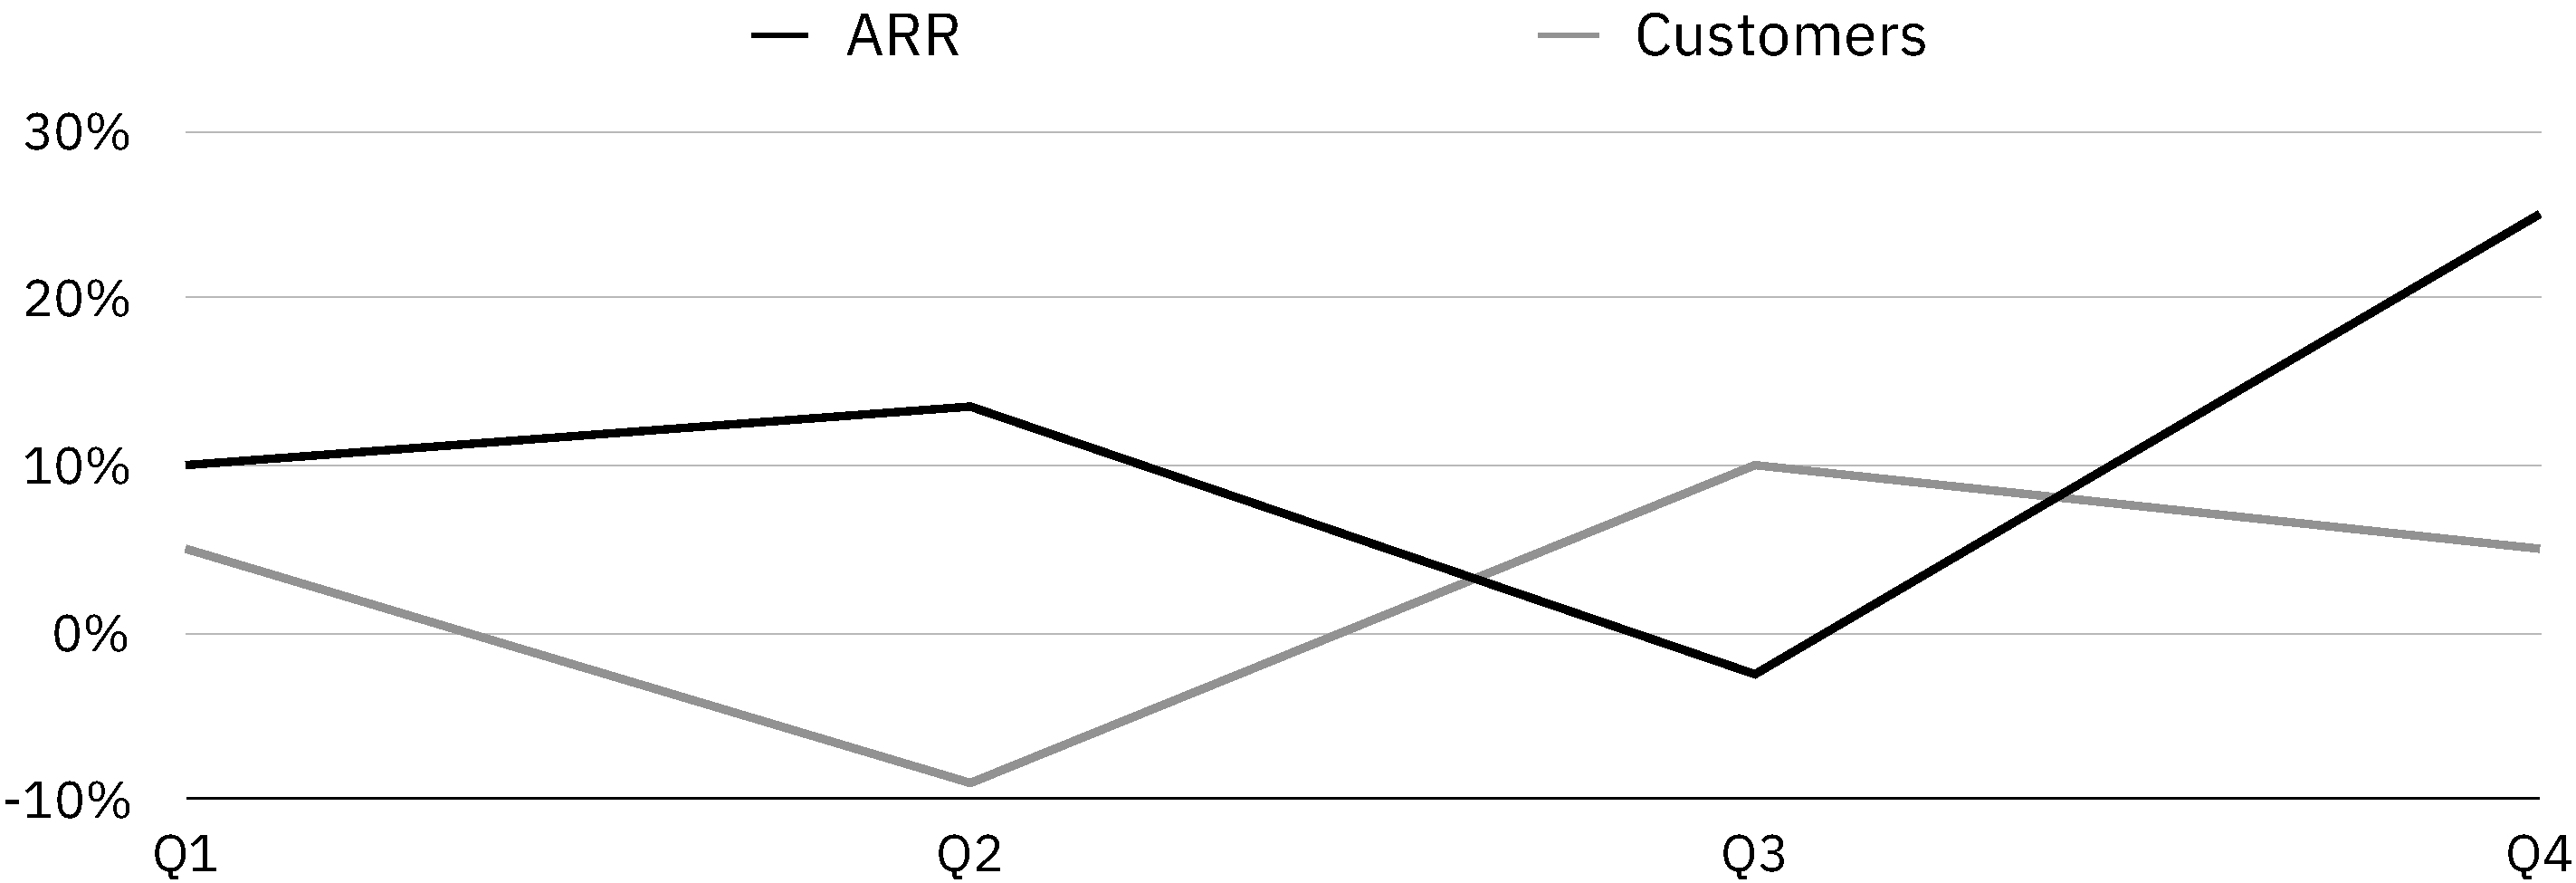
\includegraphics[width=\linewidth]{ARR.pdf}
	\caption{Text block figure caption.}
	\label{fig:example} % Label for referencing this figure in the text automatically
\end{figure}

%------------------------------------------------

\begin{figure*} % Use the figure* environment for full width figures
	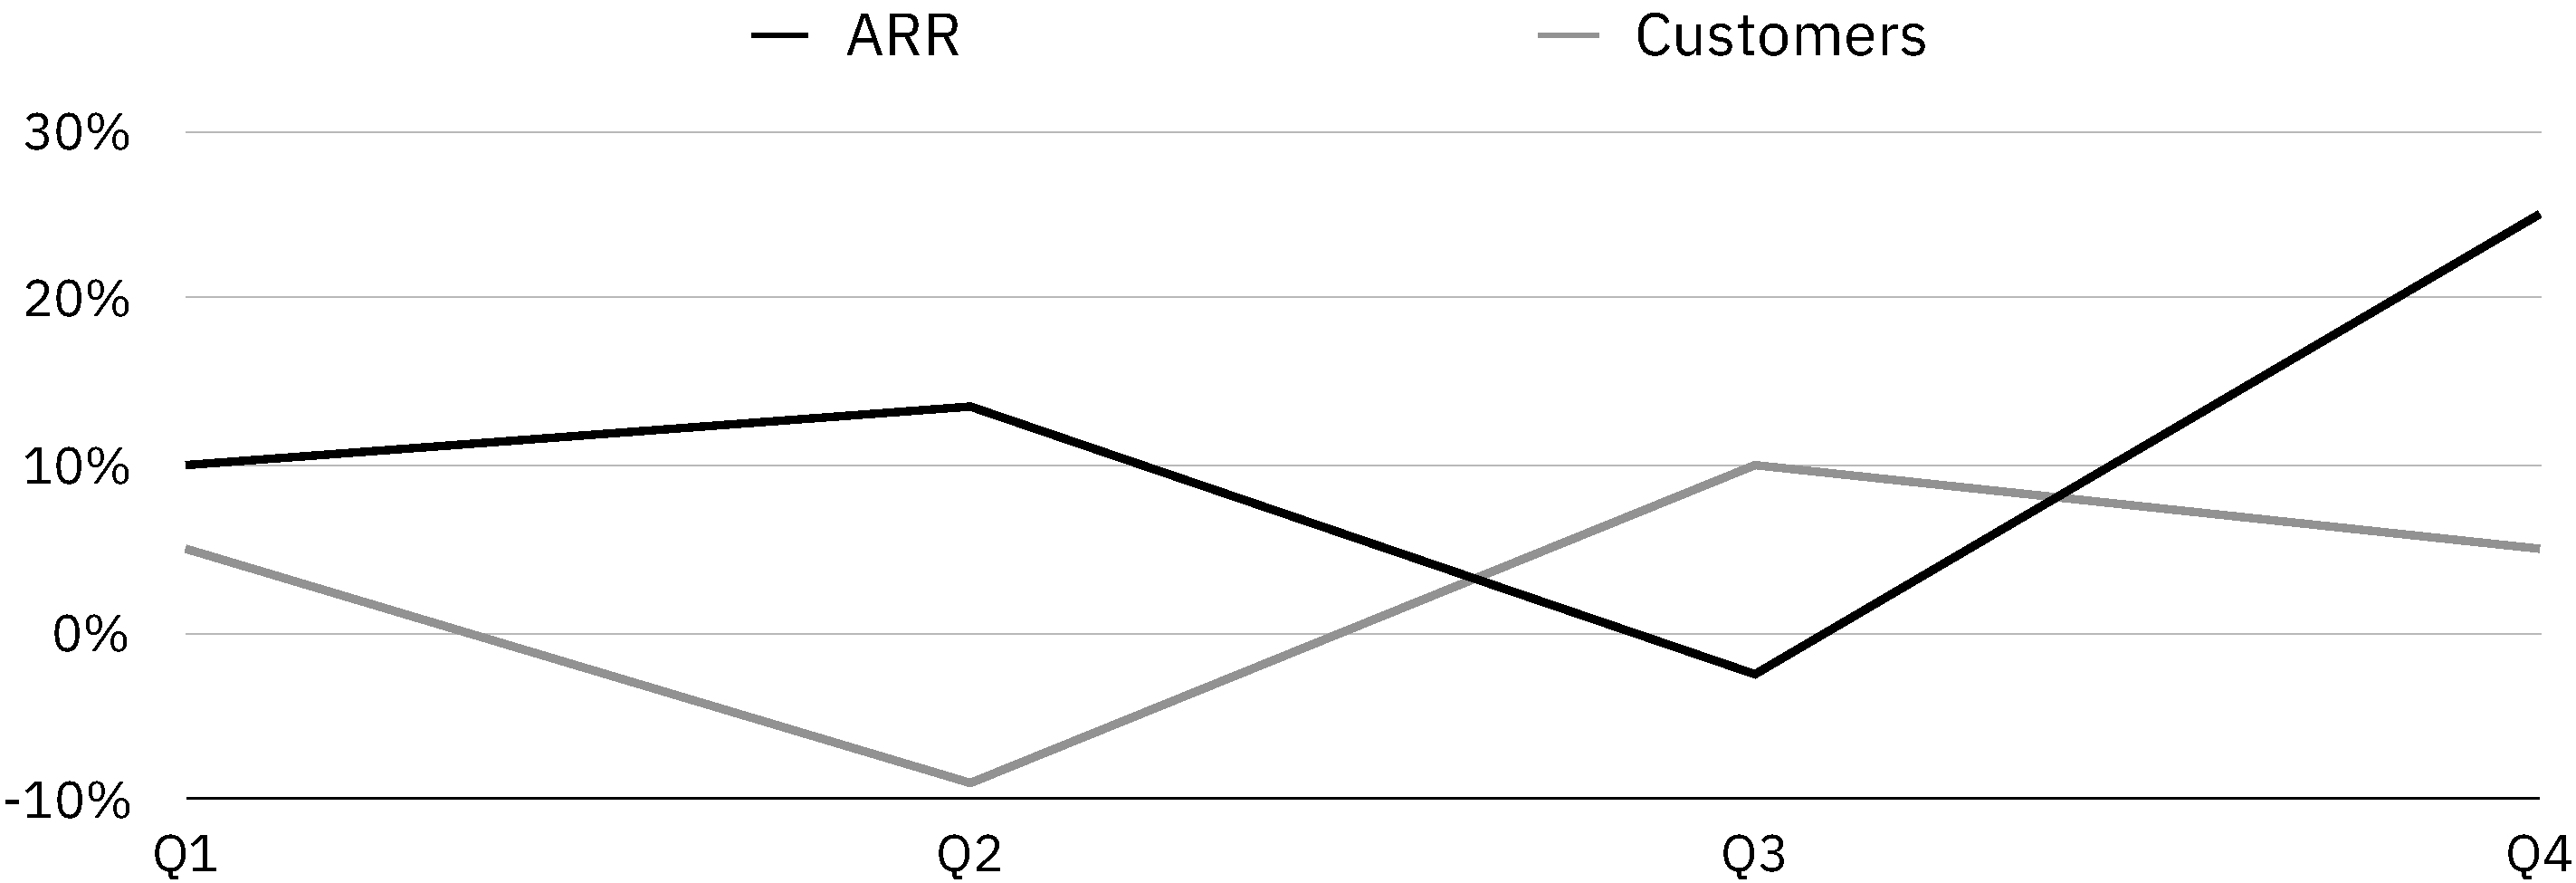
\includegraphics[width=\linewidth]{ARR.pdf}
	\caption{Full width figure caption.}
\end{figure*}

%----------------------------------------------------------------------------------------
%	LISTS
%----------------------------------------------------------------------------------------

\section{List Examples}

\subsection{Bullet Point List}

\nonumsidenote{Bullet point lists can also be created in the margin. For these, we can remove the usual left margin to increase the available horizontal space:\\\medskip \begin{itemize}[leftmargin=*]\item Bullet item one. \item Bullet item two. \item Bullet item three.\end{itemize}}Lorem ipsum dolor sit amet, consectetur adipiscing elit. Praesent porttitor arcu luctus, imperdiet urna iaculis, mattis eros. Pellentesque iaculis odio vel nisl ullamcorper, nec faucibus ipsum molestie. Sed dictum nisl non aliquet porttitor.

\begin{itemize}
	\item First bullet point item
	\begin{itemize}
		\item First indented bullet point item
		\item Second indented bullet point item
		\begin{itemize}
			\item First second-level indented bullet point item
			\item Second second-level indented bullet point item
		\end{itemize}
		\item Third indented bullet point item
	\end{itemize}
	\item Second bullet point item
	\item Third bullet point item
\end{itemize}

Etiam vulputate arcu dignissim, finibus sem et, viverra nisl. Aenean luctus congue massa, ut laoreet metus ornare in. Nunc fermentum nisi imperdiet lectus tincidunt vestibulum at ac elit. Nulla mattis nisl eu malesuada suscipit.

%------------------------------------------------

\subsection{Numbered List}

\nonumsidenote[-2.5cm]{Numbered lists can also be created in the margin. For these, we can remove the usual left margin to increase the available horizontal space:\\\medskip \begin{enumerate}[leftmargin=*]\item Numbered item one. \item Numbered item two. \item Numbered item three.\end{enumerate}}Lorem ipsum dolor sit amet, consectetur adipiscing elit. Praesent porttitor arcu luctus, imperdiet urna iaculis, mattis eros. Pellentesque iaculis odio vel nisl ullamcorper, nec faucibus ipsum molestie. Sed dictum nisl non aliquet porttitor.

\begin{enumerate}
	\item First numbered item
	\begin{enumerate}
		\item First indented numbered item
		\item Second indented numbered item
		\begin{enumerate}
			\item First second-level indented numbered item
			\item Second second-level indented numbered item
		\end{enumerate}
		\item Third indented numbered item
	\end{enumerate}
	\item Second numbered item
	\item Third numbered item
\end{enumerate}

Etiam vulputate arcu dignissim, finibus sem et, viverra nisl. Aenean luctus congue massa, ut laoreet metus ornare in. Nunc fermentum nisi imperdiet lectus tincidunt vestibulum at ac elit. Nulla mattis nisl eu malesuada suscipit.

%------------------------------------------------

\subsection{Description List}

\nonumsidenote{Description lists can also be created in the margin:\\\medskip \begin{description}\item[A1] Description item one. \item[B1] Description item two. \item[C1] Description item three.\end{description}}Lorem ipsum dolor sit amet, consectetur adipiscing elit. Praesent porttitor arcu luctus, imperdiet urna iaculis, mattis eros. Pellentesque iaculis odio vel nisl ullamcorper, nec faucibus ipsum molestie. Sed dictum nisl non aliquet porttitor.

\begin{description}
	\item[Item One] Lorem ipsum dolor sit amet, consectetur adipiscing elit. Praesent porttitor arcu luctus, imperdiet urna iaculis, mattis eros. Pellentesque iaculis odio vel nisl ullamcorper, nec faucibus ipsum molestie.
	\item[Item Two] Sed dictum nisl non aliquet porttitor.
	\begin{description}
		\item[Subitem] Maecenas consectetur metus at tellus finibus condimentum. Proin arcu lectus, ultrices non tincidunt et, tincidunt ut quam. Integer luctus posuere est, non maximus ante dignissim quis.
		\begin{description}
			\item[Subsubitem] Maecenas consectetur metus at tellus finibus condimentum. Proin arcu lectus, ultrices non tincidunt et, tincidunt ut quam. Integer luctus posuere est, non maximus ante dignissim quis.
	\end{description}
	\end{description}
	\item[Item Three] Etiam vulputate arcu dignissim, finibus sem et, viverra nisl. Aenean luctus congue massa, ut laoreet metus ornare in. Nunc fermentum nisi imperdiet lectus tincidunt vestibulum at ac elit. Nulla mattis nisl eu malesuada suscipit.
\end{description}

Etiam vulputate arcu dignissim, finibus sem et, viverra nisl. Aenean luctus congue massa, ut laoreet metus ornare in.

%----------------------------------------------------------------------------------------
%	REFERENCING CITATIONS
%----------------------------------------------------------------------------------------

\section{Referencing Citations}

This statement requires citation \autocite{Smith:2024jd}.

This statement requires multiple citations \autocite{Smith:2024jd, Smith:2023qr}.

This short citation is in the margin\sidecite{Smith:2023qr}.

This long citation is in the margin\fullsidecite{Smith:2024jd}.

This statement has an in-text citation: \textcite{Smith:2024jd}.

%----------------------------------------------------------------------------------------
%	LINKS
%----------------------------------------------------------------------------------------

\section{Link Examples}

This is a URL link: \href{https://www.duckduckgo.com}{DuckDuckGo}.\nonumsidenote{Links can be clicked in the PDF to navigate to the linked website or email address.}

This is a email link: \href{mailto:example@example.com}{example@example.com}.

This is a monospaced URL link: \url{https://duckduckgo.com}.

%----------------------------------------------------------------------------------------
%	EQUATIONS
%----------------------------------------------------------------------------------------

\section{Equation}

\begin{equation}
	\cos^3 \theta =\frac{1}{4}\cos\theta+\frac{3}{4}\cos 3\theta
	\label{eq:example}
\end{equation}

This statement automatically references the equation above using its label: Equation \ref{eq:example}.

%----------------------------------------------------------------------------------------
%	INTERNATIONAL SUPPORT
%----------------------------------------------------------------------------------------

\section{International Support}

àáâäãåèéêëìíîïòóôöõøùúûüÿýñçčšž\nonumsidenote{Plex is a very high quality typeface produced by IBM. It includes extensive international support and characters.}

ÀÁÂÄÃÅÈÉÊËÌÍÎÏÒÓÔÖÕØÙÚÛÜŸÝÑ

ßÇŒÆČŠŽ

%----------------------------------------------------------------------------------------
%	CODE
%----------------------------------------------------------------------------------------

\section{Displaying Code}

The block below is a code listing. It displays code in an easy to use way with line numbers for quick reference to specific parts of the code.

\begin{lstlisting}
{
	"city": [
		{
			"id": 1,
			"name": "Toronto",
			"country": "Canada",
			"population": 6200000
		},
		{
			"id": 2,
			"name": "New York",
			"country": "United States of America",
			"population": 8800000
		}
	]
}
\end{lstlisting}

%----------------------------------------------------------------------------------------
%	 REFERENCES/BIBLIOGRAPHY
%----------------------------------------------------------------------------------------

\newpage

\addcontentsline{toc}{section}{Reference List} % Add the bibliography to the table of contents

\begin{twothirdswidth} % Content in this environment to be at two-thirds of the whole page width
	\printbibliography[title=Reference List] % Output the bibliography with a custom section title
\end{twothirdswidth}

%----------------------------------------------------------------------------------------
%	APPENDICES
%----------------------------------------------------------------------------------------

\newpage

\section*{Appendices}

\begin{appendices}

\section{Appendix Section}

Lorem ipsum dolor sit amet, consectetur adipiscing elit. Aliquam auctor mi risus, quis tempor libero hendrerit at. Duis hendrerit placerat quam et semper. Nam ultricies metus vehicula arcu viverra, vel ullamcorper justo elementum. Pellentesque vel mi ac lectus cursus posuere et nec ex. Fusce quis mauris egestas lacus commodo venenatis. Ut at arcu lectus. Donec et urna nunc. Morbi eu nisl cursus sapien eleifend tincidunt quis quis est. Donec ut orci ex. Praesent ligula enim, ullamcorper non lorem a, ultrices volutpat dolor. Nullam at imperdiet urna. Pellentesque nec velit eget euismod pretium.

\section{Appendix Section}

Lorem ipsum dolor sit amet, consectetur adipiscing elit. Aliquam auctor mi risus, quis tempor libero hendrerit at. Duis hendrerit placerat quam et semper. Nam ultricies metus vehicula arcu viverra, vel ullamcorper justo elementum. Pellentesque vel mi ac lectus cursus posuere et nec ex. Fusce quis mauris egestas lacus commodo venenatis. Ut at arcu lectus. Donec et urna nunc. Morbi eu nisl cursus sapien eleifend tincidunt quis quis est. Donec ut orci ex. Praesent ligula enim, ullamcorper non lorem a, ultrices volutpat dolor. Nullam at imperdiet urna. Pellentesque nec velit eget euismod pretium.

\section{Appendix Section}

Lorem ipsum dolor sit amet, consectetur adipiscing elit. Aliquam auctor mi risus, quis tempor libero hendrerit at. Duis hendrerit placerat quam et semper. Nam ultricies metus vehicula arcu viverra, vel ullamcorper justo elementum. Pellentesque vel mi ac lectus cursus posuere et nec ex. Fusce quis mauris egestas lacus commodo venenatis. Ut at arcu lectus. Donec et urna nunc. Morbi eu nisl cursus sapien eleifend tincidunt quis quis est. Donec ut orci ex. Praesent ligula enim, ullamcorper non lorem a, ultrices volutpat dolor. Nullam at imperdiet urna. Pellentesque nec velit eget euismod pretium.

\end{appendices}

%----------------------------------------------------------------------------------------

\end{document}
